% Figure 5.1: System Architecture Diagram
% Compile with: pdflatex fig_5_1_system_architecture.tex

\documentclass[border=10pt]{standalone}
\usepackage{tikz}
\usetikzlibrary{shapes.geometric, arrows.meta, positioning, fit, backgrounds}
\usepackage{xcolor}

% Professional academic color palette (muted, grayscale-friendly)
\definecolor{layer1}{RGB}{70, 130, 180}    % Steel blue
\definecolor{layer2}{RGB}{100, 149, 237}   % Cornflower blue
\definecolor{layer3}{RGB}{119, 136, 153}   % Light slate gray
\definecolor{layer4}{RGB}{112, 128, 144}   % Slate gray
\definecolor{accentcolor}{RGB}{47, 79, 79} % Dark slate gray
\definecolor{bglight}{RGB}{245, 245, 245}  % White smoke
\definecolor{textdark}{RGB}{33, 33, 33}    % Near black

\begin{document}
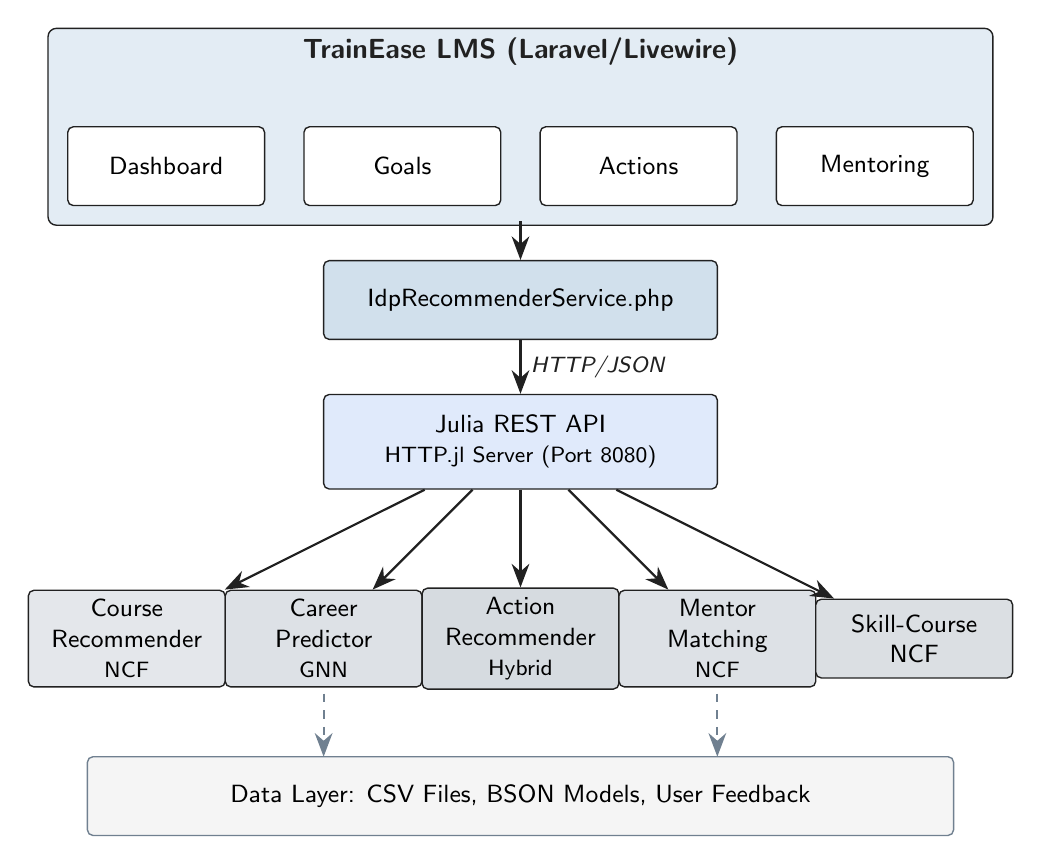
\begin{tikzpicture}[
    node distance=1.5cm,
    box/.style={rectangle, draw=textdark, rounded corners=2pt, minimum width=2.5cm, minimum height=1cm, align=center, font=\small\sffamily, line width=0.5pt},
    bigbox/.style={rectangle, draw=textdark, rounded corners=3pt, minimum width=12cm, minimum height=2.5cm, align=center, line width=0.5pt},
    arrow/.style={-{Stealth[length=3mm]}, thick, color=textdark},
    label/.style={font=\footnotesize\sffamily\itshape, color=textdark}
]

% TrainEase Layer (Laravel)
\node[bigbox, fill=layer1!15] (trainease) at (0, 3) {};
\node[font=\bfseries\sffamily, anchor=north, color=textdark] at (trainease.north) {TrainEase LMS (Laravel/Livewire)};

\node[box, fill=white] (dashboard) at (-4.5, 2.5) {Dashboard};
\node[box, fill=white] (goals) at (-1.5, 2.5) {Goals};
\node[box, fill=white] (actions) at (1.5, 2.5) {Actions};
\node[box, fill=white] (mentoring) at (4.5, 2.5) {Mentoring};

% Service Layer
\node[box, fill=layer1!25, minimum width=5cm] (service) at (0, 0.8) {IdpRecommenderService.php};

% Arrow from TrainEase to Service
\draw[arrow] (0, 1.8) -- (service);

% API Layer
\node[box, fill=layer2!20, minimum width=5cm, minimum height=1.2cm] (api) at (0, -1) {Julia REST API\\{\footnotesize\sffamily HTTP.jl Server (Port 8080)}};

% Arrow from Service to API
\draw[arrow] (service) -- node[right, label] {HTTP/JSON} (api);

% Model Layer
\node[box, fill=layer3!20] (course) at (-5, -3.5) {Course\\Recommender\\{\footnotesize\sffamily NCF}};
\node[box, fill=layer3!25] (career) at (-2.5, -3.5) {Career\\Predictor\\{\footnotesize\sffamily GNN}};
\node[box, fill=layer3!30] (action) at (0, -3.5) {Action\\Recommender\\{\footnotesize\sffamily Hybrid}};
\node[box, fill=layer3!25] (mentor) at (2.5, -3.5) {Mentor\\Matching\\{\footnotesize\sffamily NCF}};
\node[box, fill=layer4!25] (skill) at (5, -3.5) {Skill-Course\\NCF};

% Arrows from API to Models
\draw[arrow] (api) -- (course);
\draw[arrow] (api) -- (career);
\draw[arrow] (api) -- (action);
\draw[arrow] (api) -- (mentor);
\draw[arrow] (api) -- (skill);

% Data Layer
\node[box, fill=bglight, draw=layer4, minimum width=11cm] (data) at (0, -5.5) {Data Layer: CSV Files, BSON Models, User Feedback};

% Arrows from Models to Data
\draw[arrow, dashed, color=layer4] (-2.5, -4.2) -- (-2.5, -5);
\draw[arrow, dashed, color=layer4] (2.5, -4.2) -- (2.5, -5);

\end{tikzpicture}
\end{document}
